\section{分類手法}
分類問題の説明を行う。

\subsection{Linear Discriminant Analysis}
\label{subsec:LDA}
Linear Discriminant Analysis(LDA)は統計分析において伝統的に用いられてきた歴史ある手法である。
特にBCIではCSPによる特徴量抽出の後に用いられることが多い。
LDAでは多次元データを部分区間で切り取り、部分空間で分類超平面を構築することでクラス分類を行う。
分類超平面を構築する手段を与えなければ、LDAは特徴量抽出手法としても機能する。
まず、多次元データ\(x\in \mathbb R^D\)を基底\(w \in \mathbb R^D\)へ写像すると、
以下の式で表されるスカラー値を獲得できる。
\begin{equation}
    z = w^Tx \in \mathbb R
\end{equation}
zに対してある閾値を設定し、\(z \geq -w_0\)の場合はクラス\(C_1\)とし、そうでない場合は
クラス\(C_2\)であるとすることで分類器を獲得できる。
多次元データを1次元空間へ写像した場合には多くの情報損失が生ずるが、
\(w\)の取り方を上手く調整することによって、クラス分離を行いやすい射影を選択できる。
クラス分類性能を向上させる\(w\)を得るために、まず以下のようにクラス毎の平均ベクトル\(m_1,m_2\)を定義する。
\begin{eqnarray}
    m_{1} & = & \frac{1}{|C_1|}\sum_{x\in C_1}x \nonumber \\
    m_{2} & = & \frac{1}{|C_2|}\sum_{x\in C_2}x
\end{eqnarray}
ここに、\(|C_i|\)はクラス\(C_i\)に属するデータの数である。
クラス\(C_1\)とクラス\(C_2\)の平均が射影先で大きな値となれば分離が行われやすいと想定できる。
従って、以下の距離の最大化によって分類性能が向上すると考えられる。
\begin{equation}
    d=|w^T(m_1-m_2)|
    \label{eq:dis}
\end{equation}
しかし実際にはクラス毎の平均を考慮しただけでは分類が上手く行くとは限らない(図\ref{fig:mean_dis})。
射影先での各クラスのデータの分散が大きい場合には、異なるクラスのデータが重なってしまう場合が生じるからである。
\begin{figure}
    \centering
    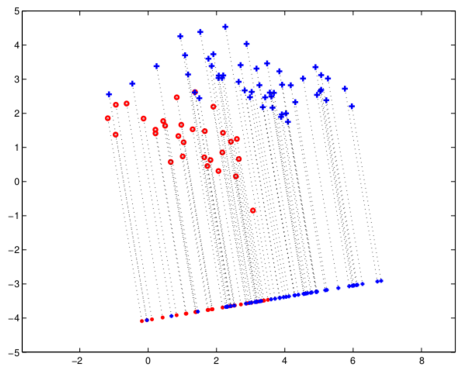
\includegraphics[width=12cm]{images/mean_dis.png}
    \caption{クラス毎の平均間の距離を射影先で最大化した判別分析}
    \label{fig:mean_dis}
\end{figure}
この問題を解決するためにはデータの分散を考慮する必要がある。
まず射影先での各クラスの分散は以下で表記できる。
\begin{eqnarray}
    \sigma^2_{1} & = & \sum_{x\in C_1}\{w^T(x-m_1)\}^2 \nonumber \\
    \sigma^2_{2} & = & \sum_{x\in C_2}\{w^T(x-m_2)\}^2
\end{eqnarray}
ここで、全データのクラス毎の分散の和を総クラス内分散として以下で定義する。
\begin{equation}
    \sigma^2  = \sigma^2_1 + \sigma^2_2
    \label{eq:sig}
\end{equation}
総クラス内分散(\ref{eq:sig})を小さくしながらクラス間の平均の距離(\ref{eq:dis})を大きくすることを考慮し
LDAでは以下の評価関数を用いる。
\begin{eqnarray}
    J(w) & = & \frac{d^2}{\sigma^2} \nonumber \\
    & = & \frac{\{w^T(m_1-m_2)\}^2}{\sum_{x\in C_1}\{w^T(x-m_1)\}^2 + \sum_{x\in C_2}\{w^T(x-m_2)\}^2}
\end{eqnarray}
このクラス間の平均とクラス内の分散を考慮した評価関数を用いることで、
射影先でデータがクラス毎に小さくまとまり、かつ異なるクラスのデータがなるべく離れるようになる(図\ref{fig:var_dis})。
\begin{figure}
    \centering
    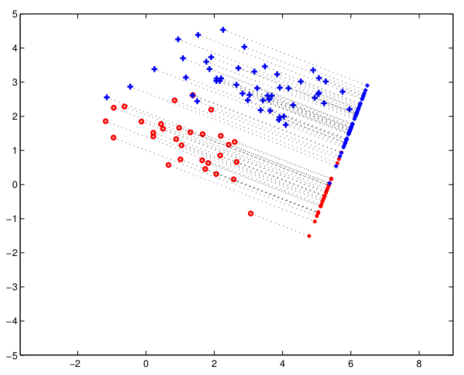
\includegraphics[width=12cm]{images/var_dis.png}
    \caption{クラス毎の平均間の距離を射影先で最大化した判別分析}
    \label{fig:var_dis}
\end{figure}

1次元の空間(数直線上)でクラス毎にデータが上手く分離できた後、
数直線上に閾値\(w_0=\frac{m_1+m_2}{2}\)を設けることで分離平面が得られる。
これはクラス毎の平均値の平均値によって分離平面を設定したことに相当する。
しかし、射影のされ方によってはこの閾値は適当ではない。
より精密な分類を行うためには、\(z=w^Tx\)がクラス毎に異なるガウス分布から生じる確率変数だと考え、
クラス\(C_i\)の条件付き確率\(p(z|C_i)\)を算出した判別基準を設け、条件付き確率が大きいクラスへ分類するなどの方法を取る。
% ガウス分布を仮定した場合における判別基準は、マハラノビス距離が近いクラスへ分類することと等価である。
% 必ずしもガウス分布であるという仮定は必要ないが、\(z\)は複数の確率変数の線型結合であるため
% 中心極限定理によりこの仮定は正当化されうる。


\subsection{Support Vector Machine}
脳波の分類ではSupport Vector Machine(SVM)の応用例もある。
基本的にSVMはマージン最大化の考えによって汎化性能の向上に成功した
2クラス分類のための線形分類器である。まずマージン最大化という概念について説明する。

マージンとは端的に述べるとデータ点と分類超平面との距離のことを表す。
学習データに対してマージンを最大化することで、学習データが空間上で僅かに移動した際にも
誤分類を起こしづらくなると期待できる。
SVMではこのマージン最大化によって以下の分類超平面を定める。
\begin{equation}
    y(x) = w^Tx + w_0
    \label{eq:displane}
\end{equation}
ここに\(x\)は\(D\)次元のデータベクトルであり、\(w\)は\(D\)次元のパラメータベクトルである。
\(w_0\)もスカラーパラメータであり閾値の役割を担う。
ここで、(\ref{eq:displane})の超平面と、あるデータ点\(x_n\)との距離は以下で表される。
\begin{equation}
    |r| = \frac{|y(x_n)|}{|w|}
    \label{eq:distance}
\end{equation}
この(\ref{eq:distance})を最大化するようにパラメータを決定することで
マージン最大化を実現することができる。
また\(x_n\)には分類面から最も近いデータ点のみを考慮すればよい。
ここで、\(x_n\)がクラス\(C_1\)に属する場合は\(t_n=1\)とし、クラス\(C_2\)に属する場合には
\(t_n=-1\)と定めた\(t_n\)を導入する。
カーネル法と組み合わせることにより非線形分類器への拡張が容易に行なえ

\subsection{Logistic Regression}
